\documentclass[conference]{IEEEtran}
\IEEEoverridecommandlockouts
% The preceding line is only needed to identify funding in the first footnote. If that is unneeded, please comment it out.
\usepackage{cite}
\usepackage{amsmath,amssymb,amsfonts}
\usepackage{graphicx}
\usepackage{textcomp}
\usepackage{xcolor}
\def\BibTeX{{\rm B\kern-.05em{\sc i\kern-.025em b}\kern-.08em
    T\kern-.1667em\lower.7ex\hbox{E}\kern-.125emX}}
\title{
\vspace{1cm}
{
\includegraphics[width=0.15\textwidth]{iithlogo.jpg} \\ Avr-GCC Assignment} }
\author{Akkugari Ruchika \\ Roll No: FWC22276 \\ akkugariruchika@gmail.com}
 \begin{document}
\maketitle
 \section {ABSTRACT}
 The information bit sequence ${1 1 1 0 1 0 1 0 1}$ is to be transmitted  by encoding with Cyclic Redundancy Check 4 $(CRC-4)$ code, for which the generator polynomial is $C(x)=x^{4}+x+1$. The encoded sequence of bits is: 
\section{COMPONENTS}
The required components list is given in Table: I. The pin out diagram of LCD is:
 \begin{figure}[h]
	 \centering
	 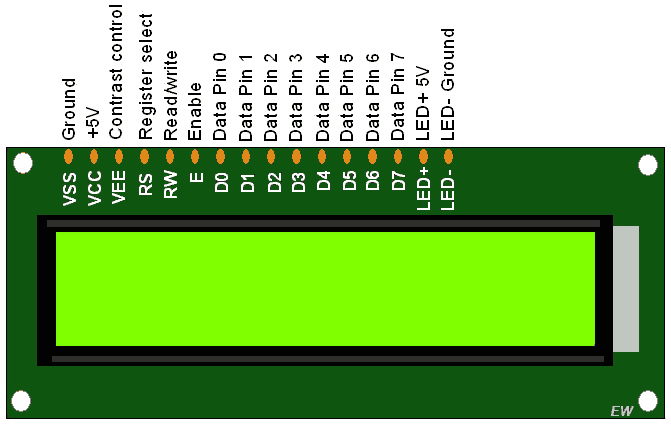
\includegraphics[width=0.35\textwidth]{lcd.png}
	 \caption{\label{fig:LCD}}
 \end{figure}
  \begin{table} [htbp]
\centering
\begin{tabular}{| c | c | c |} \hline
Components & Value & Quantity \\\hline
	LCD & $16\times2$ & 1 \\ \hline
Arduino & UNO & 1 \\ \hline
Jumper Wires &  & 20 \\ \hline
Breadboard & & 1 \\ 
\hline
\end{tabular}
\vspace{0.1cm}
\caption{\label{tab:widgets}}
\end{table}\\
\section{PROCEDURE}
To execute avr-gcc in Termux and display the output on an LCD via Arduino, first install the AVR toolchain using `pkg install avr-gcc`. Write your Arduino code in a `.c` or `.cpp` file, ensuring it initializes the LCD (using the **LiquidCrystal** library). Compile the program using $`avr-gcc -mmcu=atmega328p -DF_CPU=16000000UL -o program.elf program.c`$, then convert it to a hex file using `avr-objcopy -O ihex program.elf program.hex`.
To upload the hex file, connect Arduino to Termux using an OTG cable, and run `avrdude -c arduino -p m328p -P /dev/ttyUSB0 -b 115200 -U flash:w:program.hex`. Once uploaded, connect the LCD to Arduino as per the LiquidCrystal library’s pin configuration. Power the setup to see the output on the LCD, confirming the program's execution.
 \begin{figure}[h]
	 \centering
	 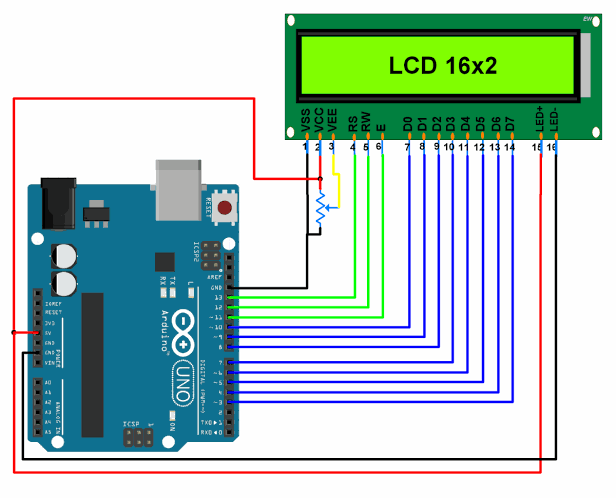
\includegraphics[width=0.35\textwidth]{connec.png}
	 \caption{\label{fig:Connections}}
 \end{figure}
\section{RESULTS}
Download the avr-gcc code given in the link below and execute them to see the output as shown in Fig.3, where the output is displayed on the LCD screen.\\
https://github.com/salad-12/FWC-INTERNSHIP/blob/main/avr-gcc/codes/avr.cpp
\begin{figure}[h] 
	\centering 
	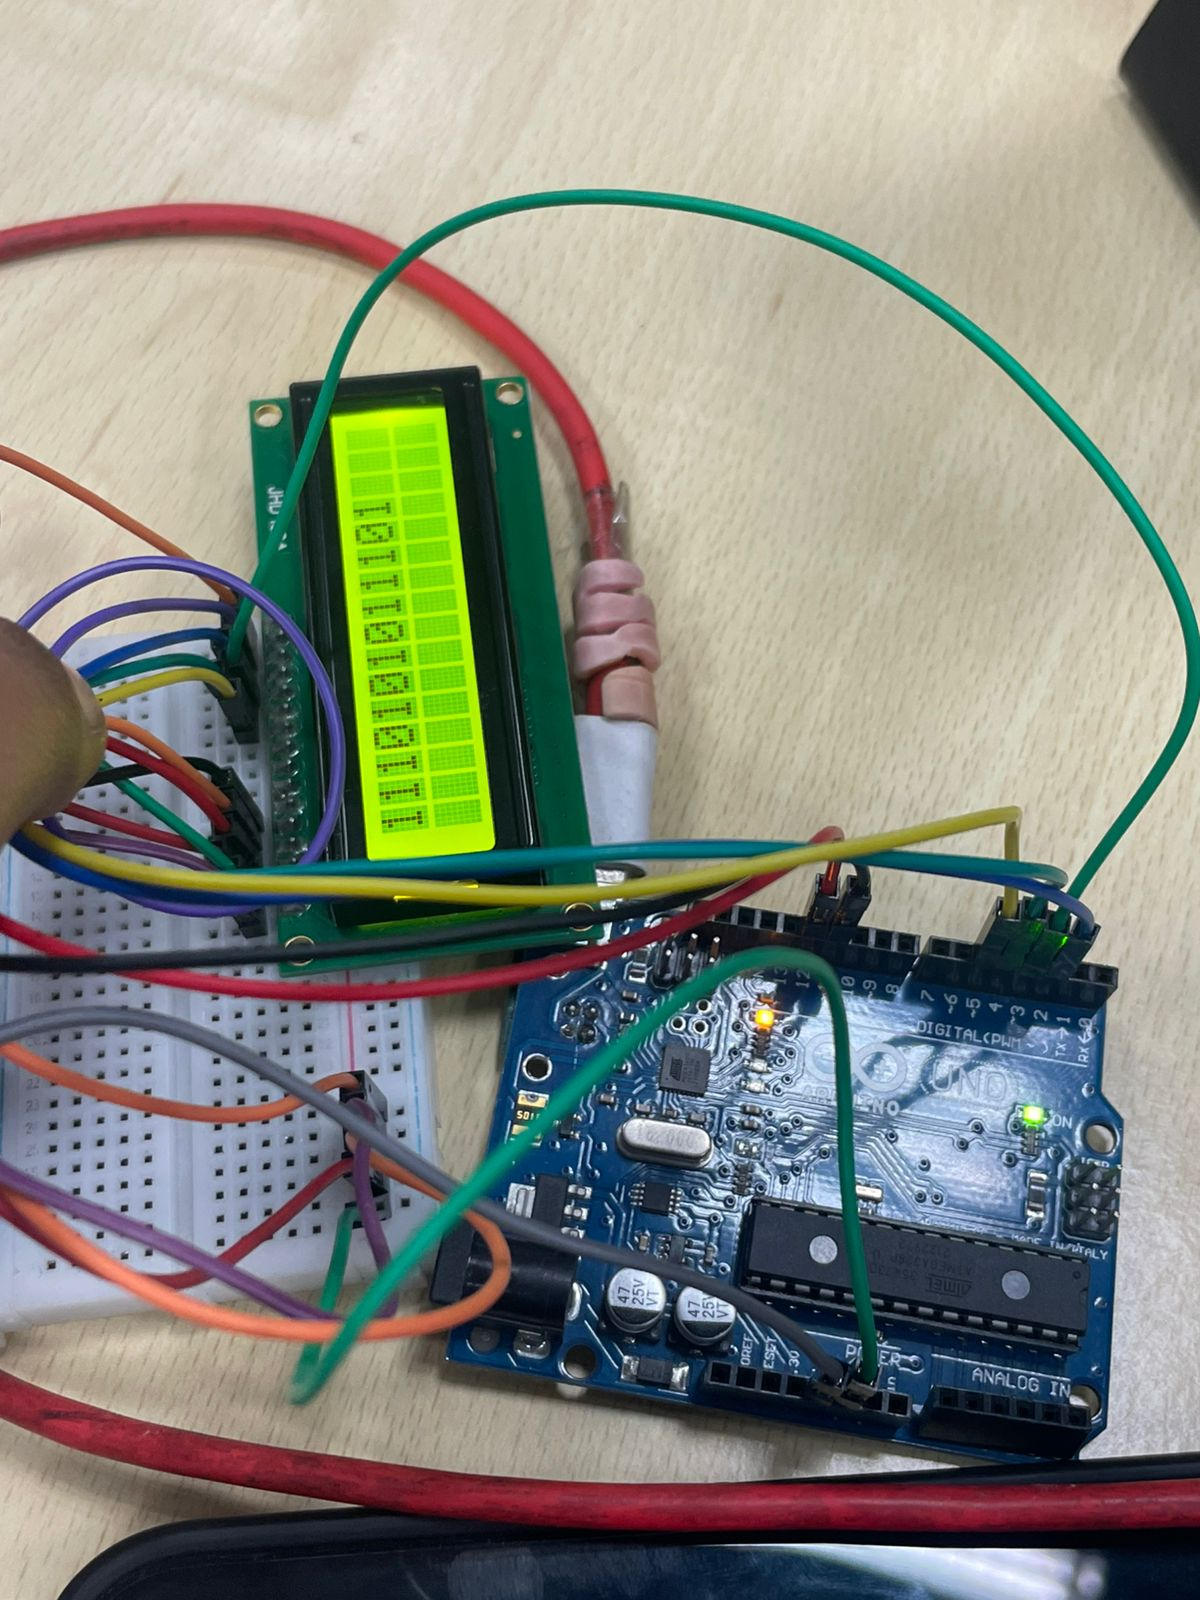
\includegraphics[width=0.4\textwidth]{avra.jpg}
	\caption{\label{fig:Result}}    
\end{figure}
\section{CONCLUSION}
In conclusion, CRC-4 (Cyclic Redundancy Check) is a robust error-detection method commonly used in digital networks to ensure data integrity by generating a 4-bit checksum. It efficiently detects errors in transmitted data, making it crucial in communication systems. On the other hand, AVR-GCC is a powerful toolchain that allows the development and compilation of programs for AVR microcontrollers, such as those used in Arduino. The combination of CRC techniques and AVR-GCC enables the creation of reliable, error-checked embedded systems, ensuring accurate data transmission and robust microcontroller programming for various applications.
\end{document}
